\documentclass[a4paper,11pt]{article}%

\usepackage{fullpage}%
\usepackage[T1]{fontenc}%
\usepackage[utf8]{inputenc}%
\usepackage[english]{babel}% % Adjust the main language

\usepackage{subcaption}

\usepackage{graphicx}%
\usepackage{url}%
\usepackage{abstract}%

\usepackage{mathpazo}%
%% Could be replaced by
%% \usepackage{newpxtext, newpxmath}
%% See the following page:
%% https://tex.stackexchange.com/questions/89610/how-to-correctly-set-up-palatino-font-with-math-related-to-pxfonts


\parskip=0.5\baselineskip

\sloppy
%% Could be replaced by  \emergencystretch 3em
%% See the following page:
%% https://tex.stackexchange.com/questions/241343/what-is-the-meaning-of-fussy-sloppy-emergencystretch-tolerance-hbadness

\begin{document}

\title{Realistic Image Synthesis \\ Assignment 1}

\author{Valentin Taillandier}

\date{\today}

\maketitle

\begin{abstract}
We made a basic ray-tracer engine in Python from scratch.
The engine supports spheres and triangles and can also load meshes in the obj format.
Since ray-tracers involve a lot of geometrical calculations, we had to implement some optimization schemes such as acceleration data-structure or tracing packs of rays with SIMD support.
\end{abstract}

\section*{Introduction}
This project is part of a course taken at the University of Tokyo which is an introduction to image synthesis.
A ray-tracer is a kind of 3D engine that traces and simulates light rays to compute colors. 
This involves various scientific fields such as Euclidean geometry (for rays intersections and reflections with objects), photometry (for color computations), and computer sciences (for computational optimization).
Not all reflection rays can be computed and, however, some heuristics exist to set the number of reflections for each ray of light.
Since a lot of rays traced from the light source are lost and do not hit the camera, we use the Fermat's backward principle to compute rays from the camera and check if the ray finally hits a light source.
This allows us to trace a fixed amount of rays defined by the resolution of the screen we are projecting the image on.
Some mandatory tasks were defined to frame the project:
\begin{description}
\item[Triangle intersection] We were provided three 3D objects defined as a set of triangles. It was natural to start by implementing triangle intersections. For each vertex of triangles,
a normal vector is provided. From that, it was also mandatory to implement barycentric normal interpolations known as Phong interpolation.
\item[Acceleration data-structure] Ray-tracers involve a lot of geometrical computations. For each pixel of the final picture, the naive way is to try to intersect a ray with each object in the scene.
A simple calculation can show that this is not computationally tractable and we had to implement a data-structure to navigate among the objects with the divide-and-conquer principle.
For personal preferences, we decided to implement BVH with SAH heuristic.
\item[Statistics] We had to provide statistics such as the number of rays traced per second or the number of object intersection tests for a pixel.
\end{description}

This report presents the state of the project, the problems we faced and provides some results.

\section{The project structure}
We adopted the Object-Oriented Programming style which is very convenient for that kind of project. Some classes come naturally:
\subsection*{The engine class}
This class (see fig.~\ref{fig:engine}) takes a centrale place in our project and links everything together.
\begin{figure}[h]
    \centering
    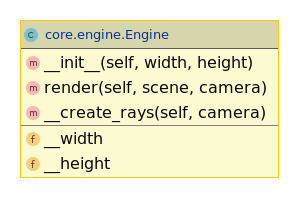
\includegraphics[scale=0.3]{img/engine.pdf}
    \caption{The engine class.}
    \label{fig:engine}
\end{figure}

The \emph{\_\_init\_\_} method is the one that is called when instantiating an object. We provide it the image's width and height in pixels.
The most important method is the \emph{render} that we call to build the picture. This method takes a scene object and a camera object computes the rays issued from the camera and returns it to the scene. For each ray, the scene computes if an object is hit and returns data about the object and the distance from the camera and the object to the engine.
The engine will then use those information to computes colors for each pixel of the picture.
\subsection*{The camera class}
This class (see fig.~\ref{fig:camera}) builds a camera object that will define the origins and directions of the rays.
\begin{figure}[h]
    \centering
    \includegraphics[scale=0.3]{img/camera.pdf}
    \caption{The camera class.}
    \label{fig:camera}
\end{figure}
The most important method here is \emph{\_\_init\_\_} used to build the camera. It takes a position point, two directional vectors (horizontal and vertical directions) and a number for the \textit{fov}.
The \textit{fov} stands for the horizontal field of view and define the angle in radiant between the rays issued for the most left and right pixels.
\subsection*{The scene and light class}
This scene class (see fig.~\ref{fig:scene}) builds an object that will store the component of the scene we want to render.
It links the engine and all of the 3D objects of the scene.
The light object builds a simple radial isotropic light source, since it is very simple we won't describe it there.
\begin{figure}[h]
    \centering
    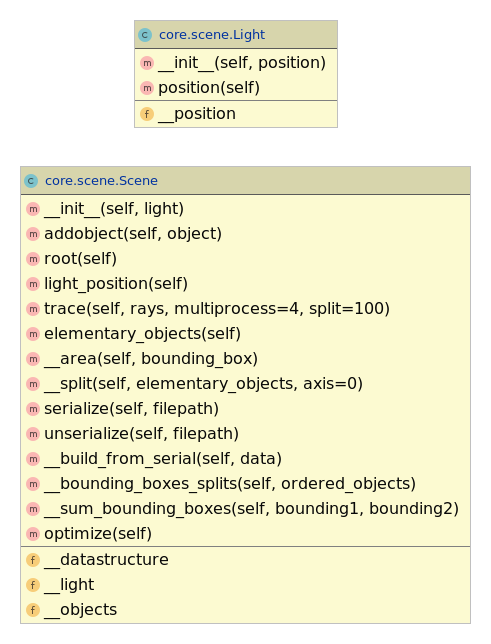
\includegraphics[scale=0.3]{img/scene.pdf}
    \caption{The scene and light class.}
    \label{fig:scene}
\end{figure}
The most important methods of the scene objects are \emph{trace}, \emph{optimize}, \emph{serialize} and \emph{unserialize}.
\emph{trace} gives the rays from the engine to every 3D objects, collects and gathers the intersection data.
\emph{optimize} is called to optimize the data-structure of objects and implement BVH and SAH.
\emph{serialize} and \emph{unserialize} are called to save and load scenes and their data-structures.
Since the \emph{optimize} method can be slow in some cases, we found it very convenient to have a way to save the work done.
The serialized scenes are simple JSON language files that reflect the tree structure of the scene.

\subsection*{The objects classes}
Several classes implement 3D objects such as triangles, spheres, groups and meshes (see fig.~\ref{fig:object}). They all inherit from a global abstract \emph{object} class.
\begin{figure}[h]
    \centering
    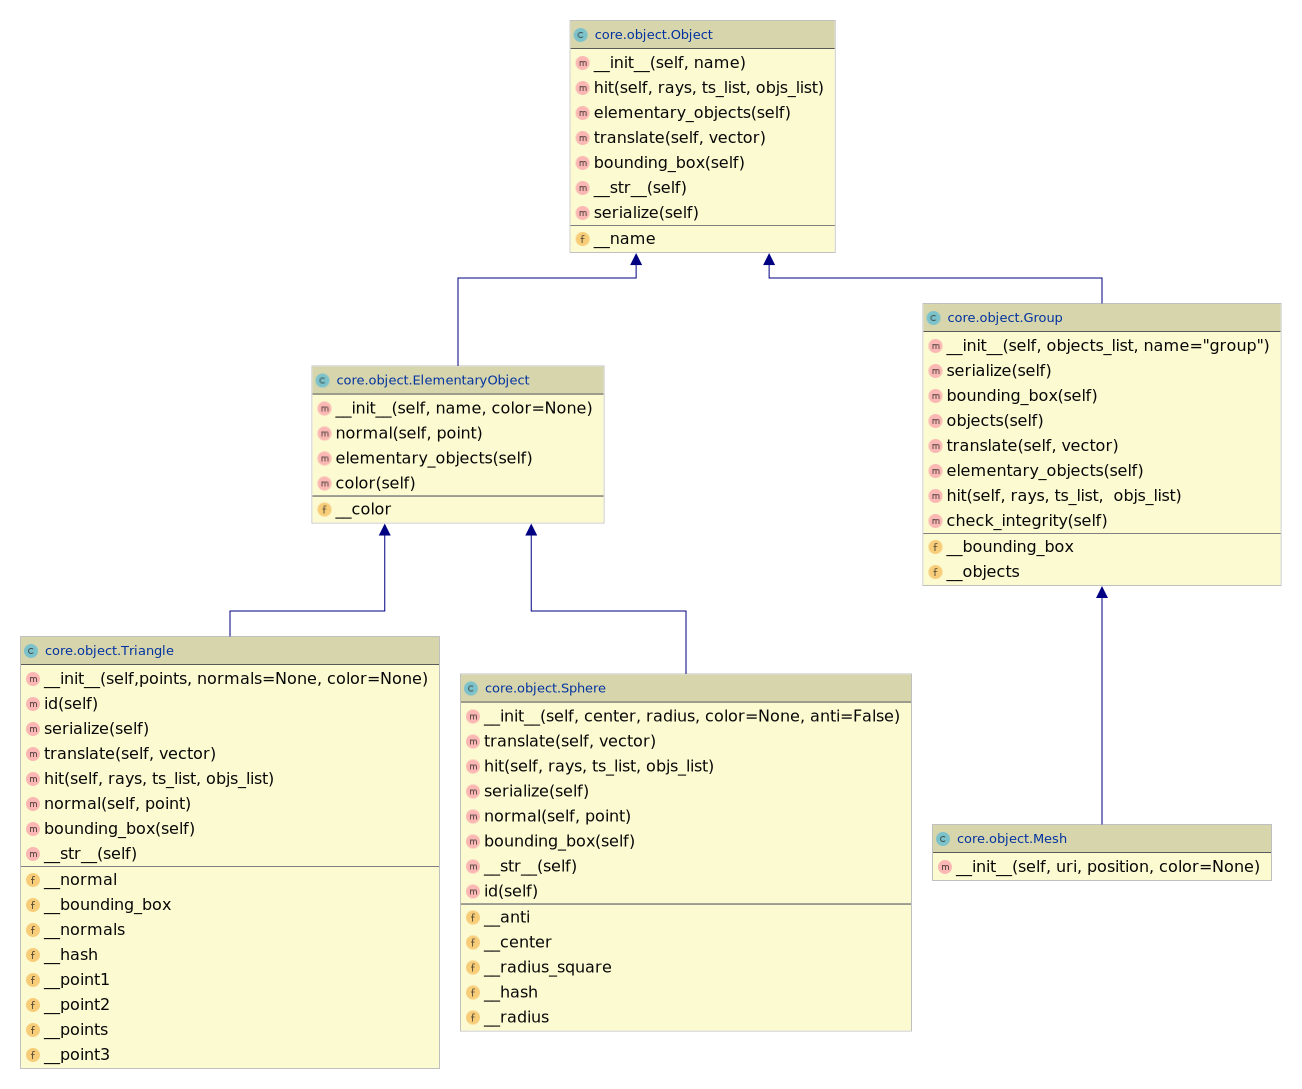
\includegraphics[scale=0.3]{img/object.pdf}
    \caption{The objects classes.}
    \label{fig:object}
\end{figure}

Two classes \emph{Group} and \emph{ElementaryObject} represent respectively the inner nodes and leaves of the tree structure of the scene.
The \textit{Group} class implements the \textit{AABB} test for the data-structure traversal while commentary objects implement their intersection methods and normal computations based on a geometrical formula.
The \emph{Mesh} class is just a special \textit{Group} class that offers a method used to load 3D objects in the .obj format.


\section{Optimization}
\subsection*{The data structure}
We decided to implement the Bounding Volume Hierarchy algorithm known as BVH to recursively split a scene into two sub-scenes.
The Surface Area Heuristic was used to select the best split from every candidate.
Some dynamic programming optimization was made to compute the candidates faster, however, the construction of the data structure is not linear in the number of objects.
Every elementary object implements a bounding box computation method that is called to get the smallest axis-aligned box that is bounding the object.
This smallest box is used by the BVH algorithm to computes the bounding box of the objects group resulting in the construction of a candidate.
The resulting data-structures can be serialized and saved to be loaded and reused later.
Figure~\ref{fig:dsteapot} shows an example of a scene rendered with a resolution of $1000\times1000$ pixels and a representation of the number of nodes traversals in the data-structure optimized by BVH.
For each pixel, we computed the number of group nodes traversed and tested elementary objects. The brighter the pixel is, the more intersection computations have been made. This representation naturally shows the
topology of the optimized data-structure. Figure~\ref{fig:dsbunny} shows the same result but for the bunny.

\begin{figure}[h]
    \centering
    
\begin{subfigure}{.5\textwidth}
  \centering
  \includegraphics[width=.9\linewidth]{img/teapot.png}
\end{subfigure}%
\begin{subfigure}{.5\textwidth}
  \centering
  \includegraphics[width=.9\linewidth]{img/tbteapot.png}
\end{subfigure}    
    
    \caption{An image rendered from the teapot 3D objects and a representation of the number of nodes traversals in the corresponding optimized data-structure.}
    \label{fig:dsteapot}
\end{figure}

\begin{figure}[h]
    \centering
    
\begin{subfigure}{.5\textwidth}
  \centering
  \includegraphics[width=.9\linewidth]{img/bunny.png}
\end{subfigure}%
\begin{subfigure}{.5\textwidth}
  \centering
  \includegraphics[width=.9\linewidth]{img/tbbunny.png}
\end{subfigure}    
    
    \caption{An image rendered from the bunny 3D objects and a representation of the number of nodes traversals in the corresponding optimized data-structure.}
    \label{fig:dsbunny}
\end{figure}

\subsection*{Packs of rays and SIMD}
We did a massive \textit{numpy} implementation that allows us to do computations with compiled C code and support of SIMD. In the modern processors, SIMD allows doing computations of 128-bits operands,
which represents four 32-bits operands computations at a time.
For each tested objects, the candidate rays are processed as a single ray.
We observed a substantial improvement in the computation duration.
\subsection*{Multithreading}
We used the \emph{multiprocessing} Python library to distribute work among every CPU's thread. For instance, with a four-core CPU, the image will be divided into 4 and every unit will compute a piece.
We faced a problem with the memory allocation used by this optimization since the scene was copied for each thread. Future work would be to use the BVH data-structure to give the relevant part of the scene to each thread. 

\section{Cosmetic}
\subsection*{Photometry}
For each pixel, we computed the brightness as a sum of the ambient, the diffuse and specular brightnesses. This is the so-called Phong's model.
The diffuse and specular brightnesses depend on the normals of the hit objects and the angle of incident and reflected rays.
Computing the reflected rays is done by applying the Descartes's law of reflection (the reflected ray is the opposite of the symmetry of the incident ray by the normal of the hit object). 
Figure~\ref{fig:lightteapot} shows the contribution of each nature of luminosities.
 

\begin{figure}[h]
    \centering
    
\begin{subfigure}{.3\textwidth}
  \centering
  \includegraphics[width=.9\linewidth]{img/ambientteapot.png}
\end{subfigure}%
\begin{subfigure}{.3\textwidth}
  \centering
  \includegraphics[width=.9\linewidth]{img/diffuseteapot.png}
\end{subfigure} %
\begin{subfigure}{.3\textwidth}
  \centering
  \includegraphics[width=.9\linewidth]{img/specularteapot.png}
\end{subfigure}    
    
    \caption{From left to right we sequentially add ambient, diffuse and specular lighting.}
    \label{fig:lightteapot}
\end{figure}

\subsubsection*{Phong interpolation}
We implemented barycentric interpolations of normals that gives a smooth aspect to surfaces composed of triangles. We computed normal maps to show improvement.
The Figure~\ref{fig:normalteapot} shows the improvement on the teapot object. The Figure~\ref{fig:normalsponza} show the same improvement for the Sponza palace.
\begin{figure}[h]
    \centering
    
\begin{subfigure}{.5\textwidth}
  \centering
  \includegraphics[width=.9\linewidth]{img/nnteapot.png}
\end{subfigure}%
\begin{subfigure}{.5\textwidth}
  \centering
  \includegraphics[width=.9\linewidth]{img/nteapot.png}
\end{subfigure}    
    
    \caption{Normal maps of the teapot with and without Phong interpolation.}
    \label{fig:normalteapot}
\end{figure}

\begin{figure}[h]
    \centering
    
\begin{subfigure}{.5\textwidth}
  \centering
  \includegraphics[width=.9\linewidth]{img/nnsponza.png}
\end{subfigure}%
\begin{subfigure}{.5\textwidth}
  \centering
  \includegraphics[width=.9\linewidth]{img/nsponza.png}
\end{subfigure}    
    
    \caption{Normal maps of the Sponza palace with and without Phong interpolation.}
    \label{fig:normalsponza}
\end{figure}
We planned to implement Phong tessellation, but the intersection test was very difficult to make and we focused on other points.

\section{Benchmark}

Four scenes were provided to make statistics on our implementation. We could not implement the scene with 20 bunnies because our implementation does not support object rotation.
However, we could recreate the three other ones. Figure~\ref{fig:benchmark} shows the recreated scenes. The images were rendered in $512\times512$ (262144 rays in total for each image).
Figure~\ref{fig:benchmarktable} shows the statistics computed.

\begin{figure}[h]
    \centering
    
\begin{subfigure}{.3\textwidth}
  \centering
  \includegraphics[width=.9\linewidth]{img/benchmarkteapot.png}
\end{subfigure}%
\begin{subfigure}{.3\textwidth}
  \centering
  \includegraphics[width=.9\linewidth]{img/benchmarkbunny.png}
\end{subfigure} %
\begin{subfigure}{.3\textwidth}
  \centering
  \includegraphics[width=.9\linewidth]{img/benchmarksponza.png}
\end{subfigure}    
    
    \caption{Three of the benchmark scenes were recreated to be compatible with our implementation.}
    \label{fig:benchmark}
\end{figure}


\begin{figure}
\centering
\small{
\begin{tabular}{c|cccccc}
     & \#Nodes    &  \#Leaves   & \#Ray traversals    & \#Triangle intersections    & Optimization (BVH)    & Rendering   \\ \hline
  Teapot  & 695 &  577 &  5845260 &  1600870 &  0sec &  5sec \\
  Bunny  & 82905 &  69452 &  1469106 &  522947 &  45sec &  26sec \\
  Sponza  & 78039 &  66454 &  44084644 &  7376469 &  43sec &  37sec \\
  
\end{tabular}
}
    \caption{Statistics made from the three rendered scenes.}
    \label{fig:benchmarktable}
\end{figure}

\end{document}



